\chapter{Stack Exchange}
\label{App:SE}
Stack Exchange data are public and regularly released. As closed communities were active between 180 and 210 days, we extracted only the first 180 days of data. Given that the first few months can be crucial for the further development of the community \cite{dover2020sustainable}, we are interested in the early evolution of Stack Exchange sites. 

Detailed information about questions, answers, and comments is available for each SE community. Each post is labelled with a unique ID, the user's ID who made the post, and the creation time. On Stack Exchange, users interact on several layers: Those interactions are considered positive.
\begin{itemize}
	\item posting an answer to the question; for every question, we extract the IDs of its answers
	\item posting a comment on the question or answer; for every question and answer, we selected the IDs of its comments
	\item accepting answer; for each question, we selected the accepted answer ID
\end{itemize}

Even though posts can be voted on and downvoted, information about a user who voted is absent, so we do not consider these interactions between users. Comments can not be downvoted, while we find only around 3\% negatively voted answers and questions, Table \ref{tab:negint}.

\begin{table}[hbt!]
	\centering
	\caption{Percentage of negatively voted interactions}
	\label{tab:negint}
	\begin{tabular}{cc|cc}
		
		\hline
		Site                        & Status & Questions & Answers \\ \hline
		\multirow{2}{*}{Physics}    & Beta   & 5\%       & 4\%     \\
		& Closed & 1\%       & 2\%     \\ \hline
		\multirow{2}{*}{Astronomy}  & Beta   & 3\%       & 3\%     \\
		& Closed & 2\%       & 1\%     \\ \hline
		\multirow{2}{*}{Economics}  & Beta   & 4\%       & 4\%     \\
		& Closed & 7\%       & 4\%     \\ \hline
		\multirow{2}{*}{Literature} & Beta   & 2\%       & 5\%     \\ 
		& Closed & 2\%       & 1\%     \\ \hline \hline
		\textbf{Average}            &        & 3.2\%     & 3\%     \\ \hline 
	\end{tabular}
\end{table}


%The data contains information about the official StackExchange reputation of each user but only as a single value measuring the final reputation of the user on the day when the data archive was released. Because of this significant shortcoming, we do not include this information in our analysis. In SE, users can give positive or negative votes to questions and answers and mark questions as a favour; however, the data is again provided as a final score recorded at the moment of the realise of the database. Since this does not allows us to analyze the evolution of scores, we omit this data from our analysis.\\


\section{Comparison between active and closed SE communities}

Table \ref{tab:site-info} compares the first 180 days between closed and active communities. Regarding basic statistics, active communities had a larger number of users, questions, answers and comments. Another simple indicator if the community will graduate or decline can be time series of active questions for seven days in Figure \ref{fig:active_questions}. The question is active if it had at least one activity, posted answer, or comment during the previous seven days. We find that live communities have more active questions after the first three months. Still, this difference is smaller for literature and astronomy. For astronomy, we observe that closed communities had more active questions in the early period of community life.


\begin{table}[h]
	\centering
	\caption[Community overview for first 180 days.]{Community overview for first 180 days, Number of users $n_u$, number of questions $n_q$, number of answers $n_a$, number of comments $n_c$}
	\label{tab:site-info}
	\begin{tabular}{llccccc}
		\toprule
		Site                 & Status                           & First Date                     & $n_u$                    & $n_q$                & $n_a$                  & $n_c$ \\ \hline
		\multirow{2}{*}{Astronomy}  & \multicolumn{1}{l|}{Closed}      & \multicolumn{1}{c|}{09/22/10} & \multicolumn{1}{c|}{336}  & \multicolumn{1}{c|}{474}  & \multicolumn{1}{c|}{953}  & 1444     \\
		& \multicolumn{1}{l|}{Beta} & \multicolumn{1}{c|}{09/24/13} & \multicolumn{1}{c|}{405}  & \multicolumn{1}{c|}{644}  & \multicolumn{1}{c|}{959}  & 2170     \\ \hline
		\multirow{2}{*}{Economics}  & \multicolumn{1}{l|}{Closed}      & \multicolumn{1}{c|}{10/11/10} & \multicolumn{1}{c|}{275}  & \multicolumn{1}{c|}{368}  & \multicolumn{1}{c|}{458}  & 1253     \\
		& \multicolumn{1}{l|}{Beta} & \multicolumn{1}{c|}{11/18/14} & \multicolumn{1}{c|}{648}  & \multicolumn{1}{c|}{1024} & \multicolumn{1}{c|}{1410} & 3553     \\ \hline
		\multirow{2}{*}{Literature} & \multicolumn{1}{l|}{Closed}      & \multicolumn{1}{c|}{02/10/10} & \multicolumn{1}{c|}{284}  & \multicolumn{1}{c|}{318}  & \multicolumn{1}{c|}{523}  & 1097     \\
		& \multicolumn{1}{l|}{Beta} & \multicolumn{1}{c|}{01/18/17} & \multicolumn{1}{c|}{478}  & \multicolumn{1}{c|}{910}  & \multicolumn{1}{c|}{907}  & 3301     \\ \hline
		\multirow{2}{*}{Physics}    & \multicolumn{1}{l|}{Closed}      & \multicolumn{1}{c|}{09/14/11} & \multicolumn{1}{c|}{281}  & \multicolumn{1}{c|}{349}  & \multicolumn{1}{c|}{564}  & 2213     \\
		& \multicolumn{1}{l|}{Launched}    & \multicolumn{1}{c|}{08/24/10} & \multicolumn{1}{c|}{1176} & \multicolumn{1}{c|}{2124} & \multicolumn{1}{c|}{4802} & 15403    \\
		\bottomrule
	\end{tabular}
\end{table}


\begin{figure}
	\centering
	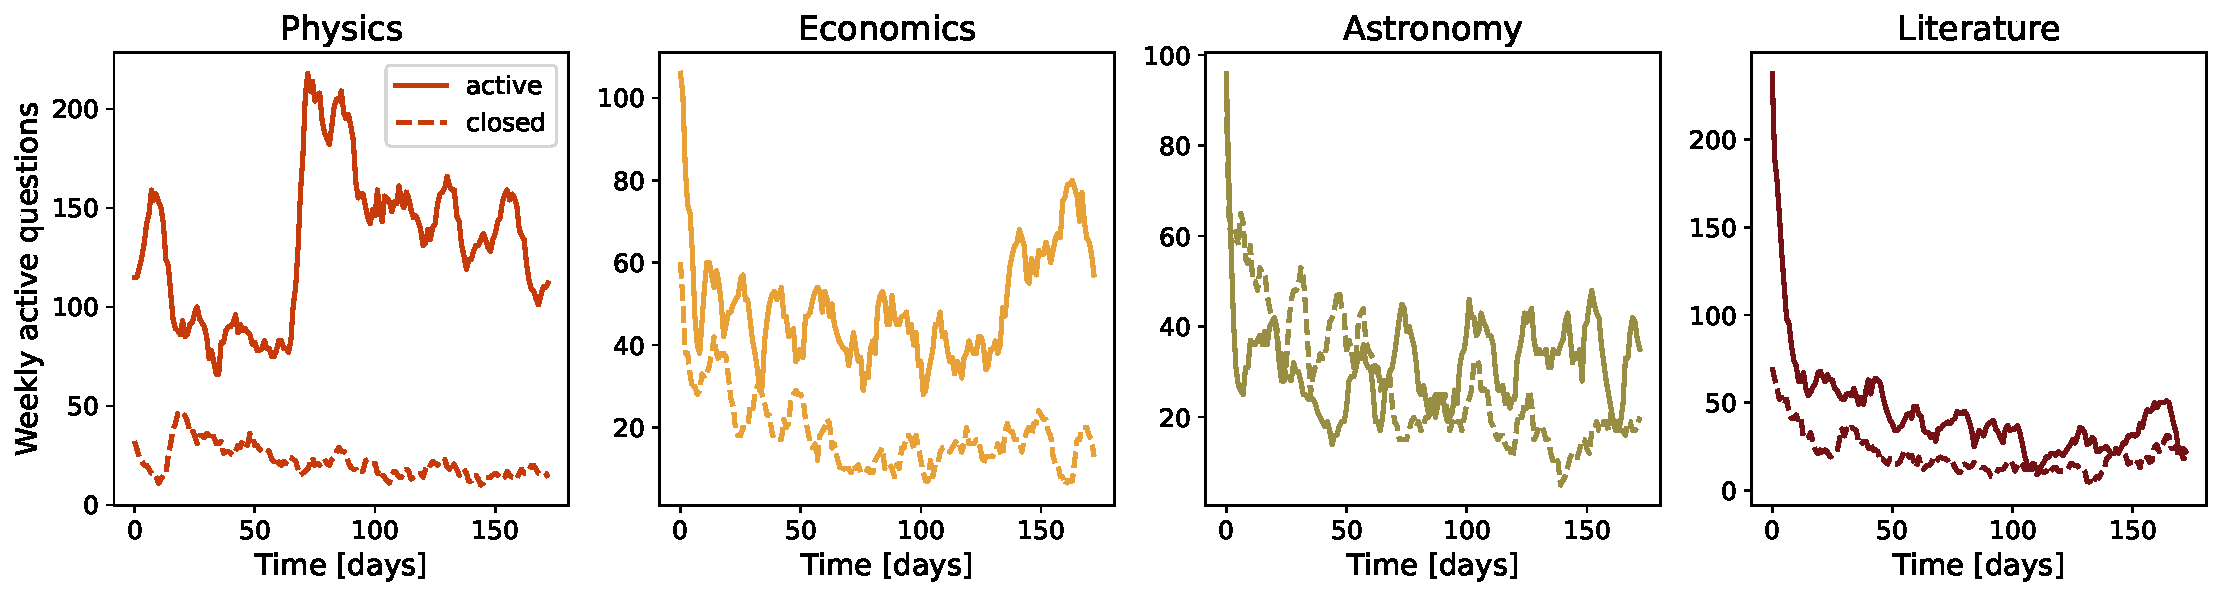
\includegraphics[width=\linewidth]{figures/stackexchange/active_questions.pdf}
	\caption[Number of active questions within seven days sliding windows]{Number of active questions within seven days sliding windows. Solid lines - active sites; dashed lines - closed sites.}
	\label{fig:active_questions}
\end{figure}

Similarly, the official Stack Exchange community evaluation process considers simple metrics \footnote{\href{https://stackoverflow.blog/2011/07/27/does-this-site-have-a-chance-of-succeeding/}{https://stackoverflow.blog/2011/07/27/does-this-site-have-a-chance-of-succeeding/}}. To determine the success of sites they measure how many questions are answered, how many questions are posted per day, and how many answers are posted per question. There are two measures: the number of avid users and the number of visits that are not easily interpreted from the data. The site is \textit{healthy} if it has ten questions per day, 2.5 answers per question and more than $90\%$ of answered questions. For less than $80\%$ of answered questions, five questions per day and 1 question per answer site \textit{needs some work}. 

We calculated Stack Exchange statistics for astronomy, economics, literature and physics and results are presented in Table \ref{tab:se_c}. After 180 days, only live physics is a healthy site while other live communities are at least in two criteria labelled as \textit{okay}. Closed sites mostly \textit{need some work}; the exception is closed astronomy. For example, it has \textit{excellent} percent of answered questions and \textit{okay} answer ratio.  

%While the Physics community was more successful than Theoretical Physics and other considered communities, these differences are not as clear if we compare three different pairs of communities. For instance, some of the parameters for a closed Astronomy community were better than for the still active community. Similar results were found for Economics and Literature. 

\begin{table}[h!]
	%\footnotesize\sf\centering
	\caption{Community overview for first 180 days according to SE criteria  }
	
	\label{tab:se_c}
	\begin{tabular}{ccccc}
		\hline
		
		Site & Status &  Answered & Questions per day & Answer ratio \\ \hline
		\multirow{2}{*}{Astronomy} & \multicolumn{1}{c|}{Closed} & \multicolumn{1}{c|}{\textbf{95} \%}  & \multicolumn{1}{c|}{2.62} & \multicolumn{1}{c}{\underline{2.02}} \\
		& \multicolumn{1}{c|}{Beta} & \multicolumn{1}{c|}{\textbf{96} \%}  & \multicolumn{1}{c|}{3.57} & \multicolumn{1}{c}{\underline{1.49}} \\ \hline
		\multirow{2}{*}{Economics} & \multicolumn{1}{c|}{Closed} & \multicolumn{1}{c|}{68 \%}  & \multicolumn{1}{c|}{2.04} & \multicolumn{1}{c}{\underline{1.25}} \\
		& \multicolumn{1}{c|}{Beta} & \multicolumn{1}{c|}{\underline{84} \%}  & \multicolumn{1}{c|}{\underline{5.66}} & \multicolumn{1}{c}{\underline{1.37}} \\ \hline
		\multirow{2}{*}{Literature} & \multicolumn{1}{c|}{Closed} & \multicolumn{1}{c|}{79 \%}  & \multicolumn{1}{c|}{1.77} & \multicolumn{1}{c}{\underline{1.65}} \\
		& \multicolumn{1}{c|}{Beta} & \multicolumn{1}{c|}{74 \%}  & \multicolumn{1}{c|}{\underline{5.04}} & \multicolumn{1}{c}{\underline{1.10}} \\ \hline
		\multirow{2}{*}{Physics} & \multicolumn{1}{c|}{Closed} & \multicolumn{1}{c|}{83 \%}  & \multicolumn{1}{c|}{1.93} & \multicolumn{1}{c}{\underline{1.64}} \\
		& \multicolumn{1}{c|}{Beta} & \multicolumn{1}{c|}{\textbf{93} \%}  & \multicolumn{1}{c|}{\textbf{11.76}} & \multicolumn{1}{c}{ \textbf{2.74}} \\ \hline \hline
		{Stack Exchange criteria} & excellent & $>$ 90 \% & $>$10 & $>$ 2.5   \\
		& needs some work & $<$ 80 \% & $<5$ & $<$ 1   \\ \hline
		
		
	\end{tabular}
	
\end{table}

These simple measurements presented in tables \ref{tab:site-info} and \ref{tab:se_c} and Figure \ref{fig:active_questions} do not provide us clear indications about community sustainability. Only for physics topics the difference between active and closed communities is evident, while for other communities, it is not so clear. Thus, we need deeper insights into the structure and dynamics of these communities to understand. The structure of social interactions within communities and the dynamics of collective trust may provide a better explanation of why some communities succeed, and others die. 